\documentclass[tikz, border=5mm]{standalone}
\usepackage{amsmath, amssymb}
\usetikzlibrary{arrows.meta, decorations.markings, calc}

\begin{document}
	
	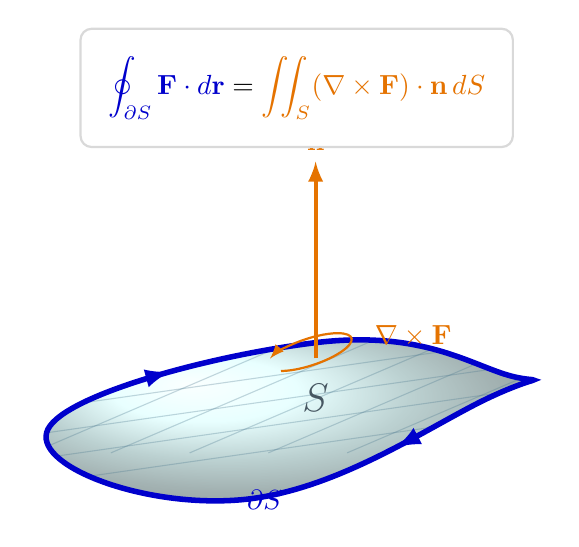
\begin{tikzpicture}[
		font=\sffamily, 
		>=latex, 
		thick,
		x={(-0.6cm,-0.4cm)}, y={(1cm,0cm)}, z={(0cm,1cm)} % 3D Coordinate system
		]
		
		% --- 1. Define the Boundary Curve (parametric ellipse-like) ---
		% We draw it in two parts: "Back" (dashed/hidden) and "Front" (solid)
		
		% Coordinates for the surface "hill"
		\def\surfpath{
			plot[smooth cycle, tension=0.8] coordinates {
				(0, 2, 0) (2, 3, 0.5) (4, 1, 0) (3, -2, 0.5) (-1, -1, 0)
			}
		}
		
		% --- 2. Draw the Surface S ---
		% We use a shading to give it 3D depth
		\shade[ball color=cyan!20, opacity=0.6] 
		plot[smooth cycle, tension=0.8] coordinates {
			(0, 2, 0) (2, 3, 0.5) (4, 1, 0) (3, -2, 0.5) (-1, -1, 0)
		};
		
		% Add a grid/mesh on the surface to emphasize curvature
		\begin{scope}
			\clip plot[smooth cycle, tension=0.8] coordinates {
				(0, 2, 0) (2, 3, 0.5) (4, 1, 0) (3, -2, 0.5) (-1, -1, 0)
			};
			\foreach \i in {-2, -1, ..., 4} {
				\draw[cyan!50!black, thin, opacity=0.3] (\i, -3, 0) -- (\i, 4, 1);
				\draw[cyan!50!black, thin, opacity=0.3] (-2, \i, 0) -- (5, \i, 1);
			}
		\end{scope}
		
		% --- 3. Draw the Boundary Loop (Front part visible) ---
		% We manually trace the "front" visible edge with arrows
		\draw[
		blue!80!black, 
		line width=2pt,
		decoration={markings, mark=at position 0.1 with {\arrow{>}}, mark=at position 0.6 with {\arrow{>}}},
		postaction={decorate}
		] 
		plot[smooth cycle, tension=0.8] coordinates {
			(0, 2, 0) (2, 3, 0.5) (4, 1, 0) (3, -2, 0.5) (-1, -1, 0)
		};
		
		% --- 4. Draw Normal Vector and Curl on the Surface ---
		% Pick a point P on the surface
		\coordinate (P) at (1.5, 0.5, 0.8); % Visually estimated "top" of the hill
		
		% Draw the Normal Vector n
		\draw[->, orange!90!black, line width=1.5pt] (P) -- ++(0, 0, 2.5) 
		node[above] {$\mathbf{n}$};
		
		% Draw the "Curl" rotation around the normal
		\begin{scope}[] 
			% This effectively draws on a plane at height z=0.8 (approx)
			% But since we are in raw 3D coords, we fake the rotation circle
			\draw[orange!90!black, thick, ->] 
			($(P) + (0.4, -0.2, 0)$) 
			arc [start angle=0, end angle=290, x radius=0.6, y radius=0.4]
			node[right=5pt, midway] {$\nabla \times \mathbf{F}$};
		\end{scope}
		
		
		% --- 5. Labels ---
		
		% Label Surface S
		\node[cyan!30!black] at (1.5, 0.5, 0.3) {\Large $S$};
		
		% Label Boundary dS
		\node[blue!80!black, anchor=west] at (4, 1, 0) {$\partial S$};
		
		% Formula Box
		\node[
		anchor=north west,
		fill=white,
		draw=gray!30,
		rounded corners,
%		drop shadow,
		inner sep=10pt
		] at (-1, -4, 4) {
			$\displaystyle 
			\color{blue!80!black} \oint_{\partial S} \mathbf{F} \cdot d\mathbf{r} 
			\color{black} = 
			\color{orange!90!black} \iint_S (\nabla \times \mathbf{F}) \cdot \mathbf{n} \, dS$
		};
		
	\end{tikzpicture}
	
\end{document}